\begin{savequote}[8cm]
\textlatin{Neque porro quisquam est qui dolorem ipsum quia dolor sit amet, consectetur, adipisci velit...}

There is no one who loves pain itself, who seeks after it and wants to have it, simply because it is pain...
  \qauthor{--- Cicero's \textit{de Finibus Bonorum et Malorum}}
\end{savequote}

\chapter{\label{ch:3-detector}The LHCb detector} 

\minitoc

The Large Hadron Collider (LHC) is the worlds largest and most powerful particle accelerator, near Geneva, Switzerland. The LHC ring is 27km in circumference, located 100m underground and consists of a series of superconducting magnets and accelerating modules to boost the particles energy. Two high energy proton or heavy ion beams travel in opposite directions at energies up to $\sqrt{s}=13\tev$. Hydrogen atoms are ionised to obtain protons, which get accelarated in stages through various parts of the LHC accelerator complex, as shown in Figure \ref{lhcdiagram}. Firstly, the protons are accelerated in Linac 2 to energies of 50\mev, followed by the Proton Syncrotron Booster (PSB), the Proton Syncrotron (PS) and the Super Proton Syncrotron (SPS), accelerating the protons to 1.4\gev, 25\gev and 450\gev respectively. Finally, they are injected into the LHC, reaching energies of up to $\sqrt{s}=13\tev$. Two proton beams are injected in opposite directions and focussed to collide at four locations around the LHC ring. These locations are where the four main particle physics detector are located, the Large Hadron Collider beauty (\lhcb) experiment as well as \atlas, \cms and \alice.

\begin{figure}
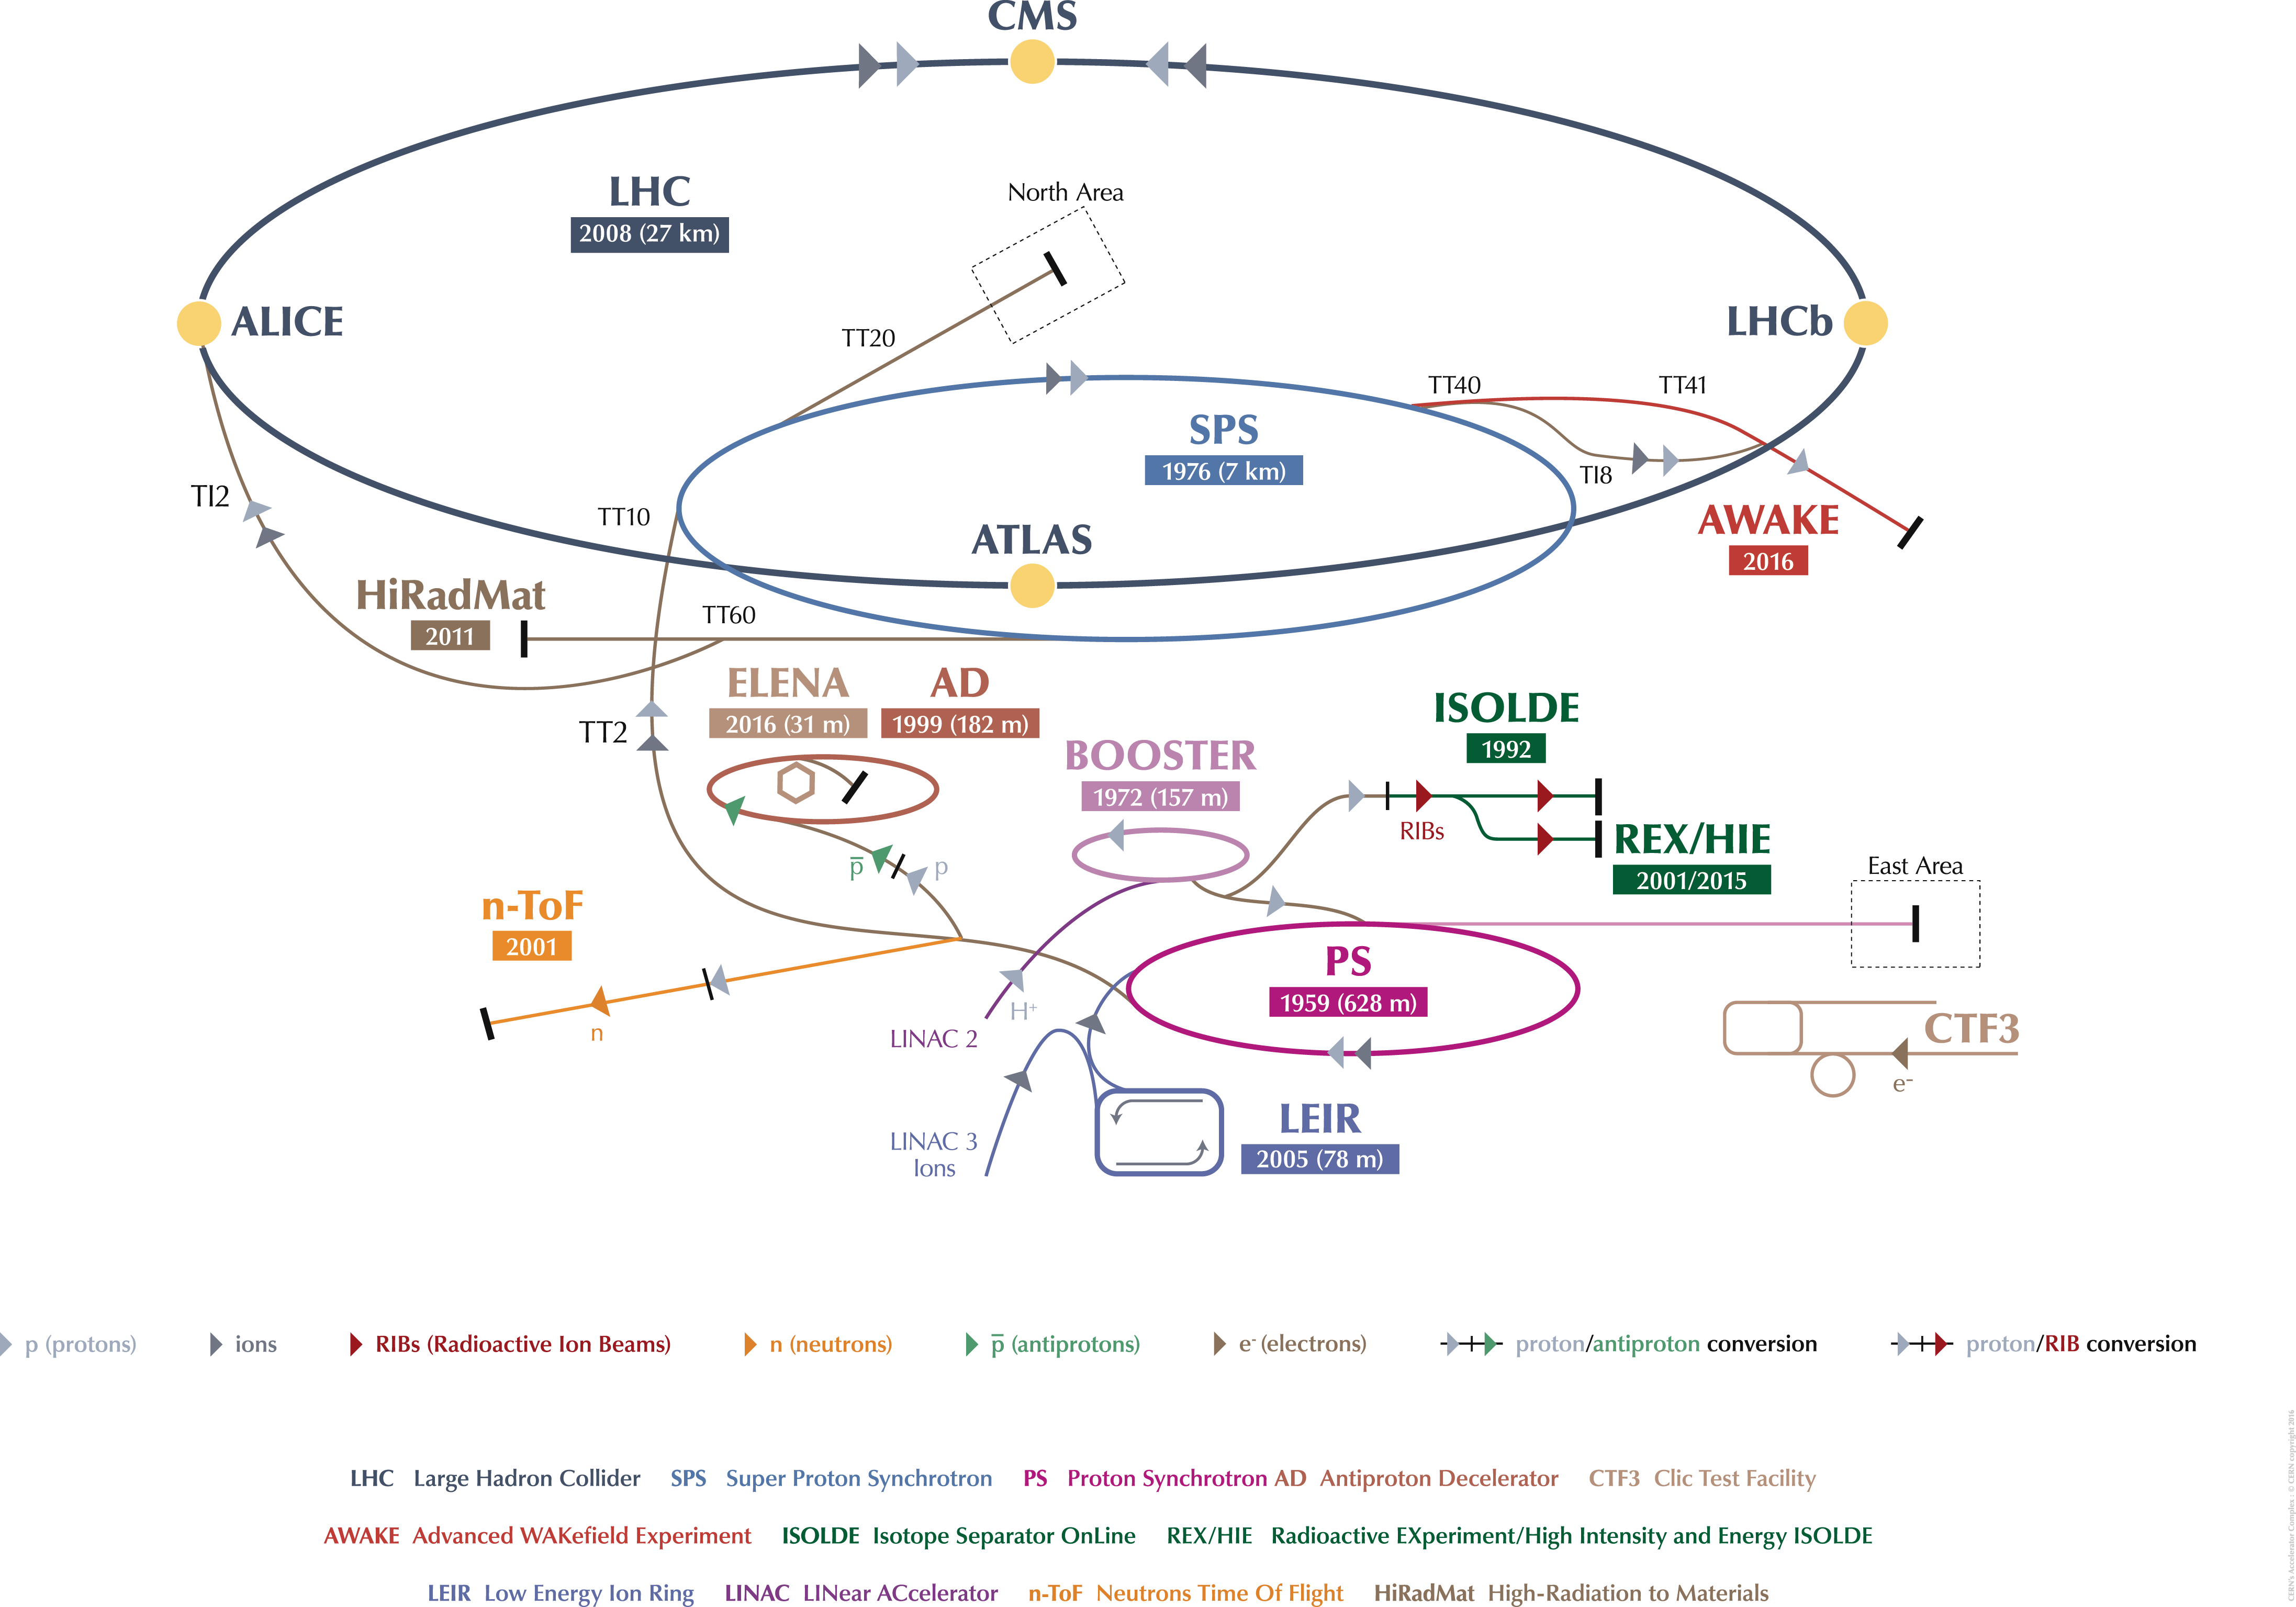
\includegraphics[width=\linewidth]{figures/detector/CCC-v2016.png}
\caption{Diagram of the LHC accelerator complex}
\label{lhcdiagram}
\end{figure}

There have been two major data taking periods of the \lhc, named \runone and \runtwo. \runone occured between 2010 and 2012, where the beam energy was $\sqrt{s}=$7\tev and 8\tev. Data collection for \runtwo began in 2015 and is due to end in 2018, with a beam energy of $\sqrt{s}=$13\tev. At LHCb the collision conditions are designed to have roughly one $pp$ interactions per bunch crossing and to limit the number of tracks. These conditions allow effective primary vertex selection, necessary for study of \B and \D meson decays, efficient processing of the track finding algorithm and reduced radiation damage and detector occupancy. This is achieved by reducing the transverse overlap of the two beams in order to reduce the area available for interactions, called luminosity levelling. It allows the peak luminosity and number of $pp$ intereactions per bunch crossing to be optimal, while maximising the intergrated luminosity. Most of the LHCb data was recorded at an instantaneous luminosity of $4 \times 10^{32}\text{cm}^{-2}\text{s}^{-1}$, with an average of 1.7 proton-proton collisions per bunch crossing for \runone and 1.1 for \runtwo. In \runone collisions occured at a frequency of 20 MHz, corresponding to collisions every 50\ns, compared to a bunch crossing rate of 40 MHz in \runtwo.

This thesis uses the whole \runonelumi \runone dataset coressponding to 1\invfb of $\sqrt{s}=$7\tev recorded in 2011 and 2\invfb of $\sqrt{s}=$8\tev recorded in 2012, as well as \runtwolumi of the \runtwo dataset, coressponding to all of the data recorded in 2015 and 2016 at $\sqrt{s}=$13\tev.

The \lhcb detector is designed to study particles containing \bquark and \cquark quarks. These quarks are produced dominantly via gluon interactions. The gluons have highly asymmetric momenta, therefore the \bquark\bquarkbar quark pair is produced predominantly in the forward (or backward) direction, as shown in Figure \ref{bbar}. For this reason, the \lhcb detector~\cite{Alves:2008zz,LHCb-DP-2014-002} is a single-arm forward spectrometer, as shown in Figure~\ref{lhcbdetector}, covering the \mbox{pseudorapidity} range $2<\eta <5$, where $\eta$ is pseudorapidity, deifned as,
\begin{equation}
\eta \equiv -\ln \left[ \tan \left( \frac{\theta}{2} \right) \right]
\end{equation}
where $\theta$ is the angle between the particles mometum vector and the beam axis. This angular region contains 25\% of \bquark\bquarkbar pairs. The detector is described using a right-handed coordinate system, where $z$ represents the direction of the beam and $x$ and $y$ are the horizontal and vertical directions. It is composed of many sub-detectors that are each specialised for a specific role. These are the Vertex Locator (\velo), the Ring Imaging Cherenkov detectors (RICH1 and RICH2), the Tracker Turicensis (TT), the dipole magnet, the tracking stations T1-T3, the calorimeter system (SPD/PS, ECAL, HCAL) and the muon stations M1-M5. In Sections \ref{sec:detector:velo} to \ref{sec:detector:muon} individual descriptions of these sub-detectors are presented.

\begin{figure}
\centering
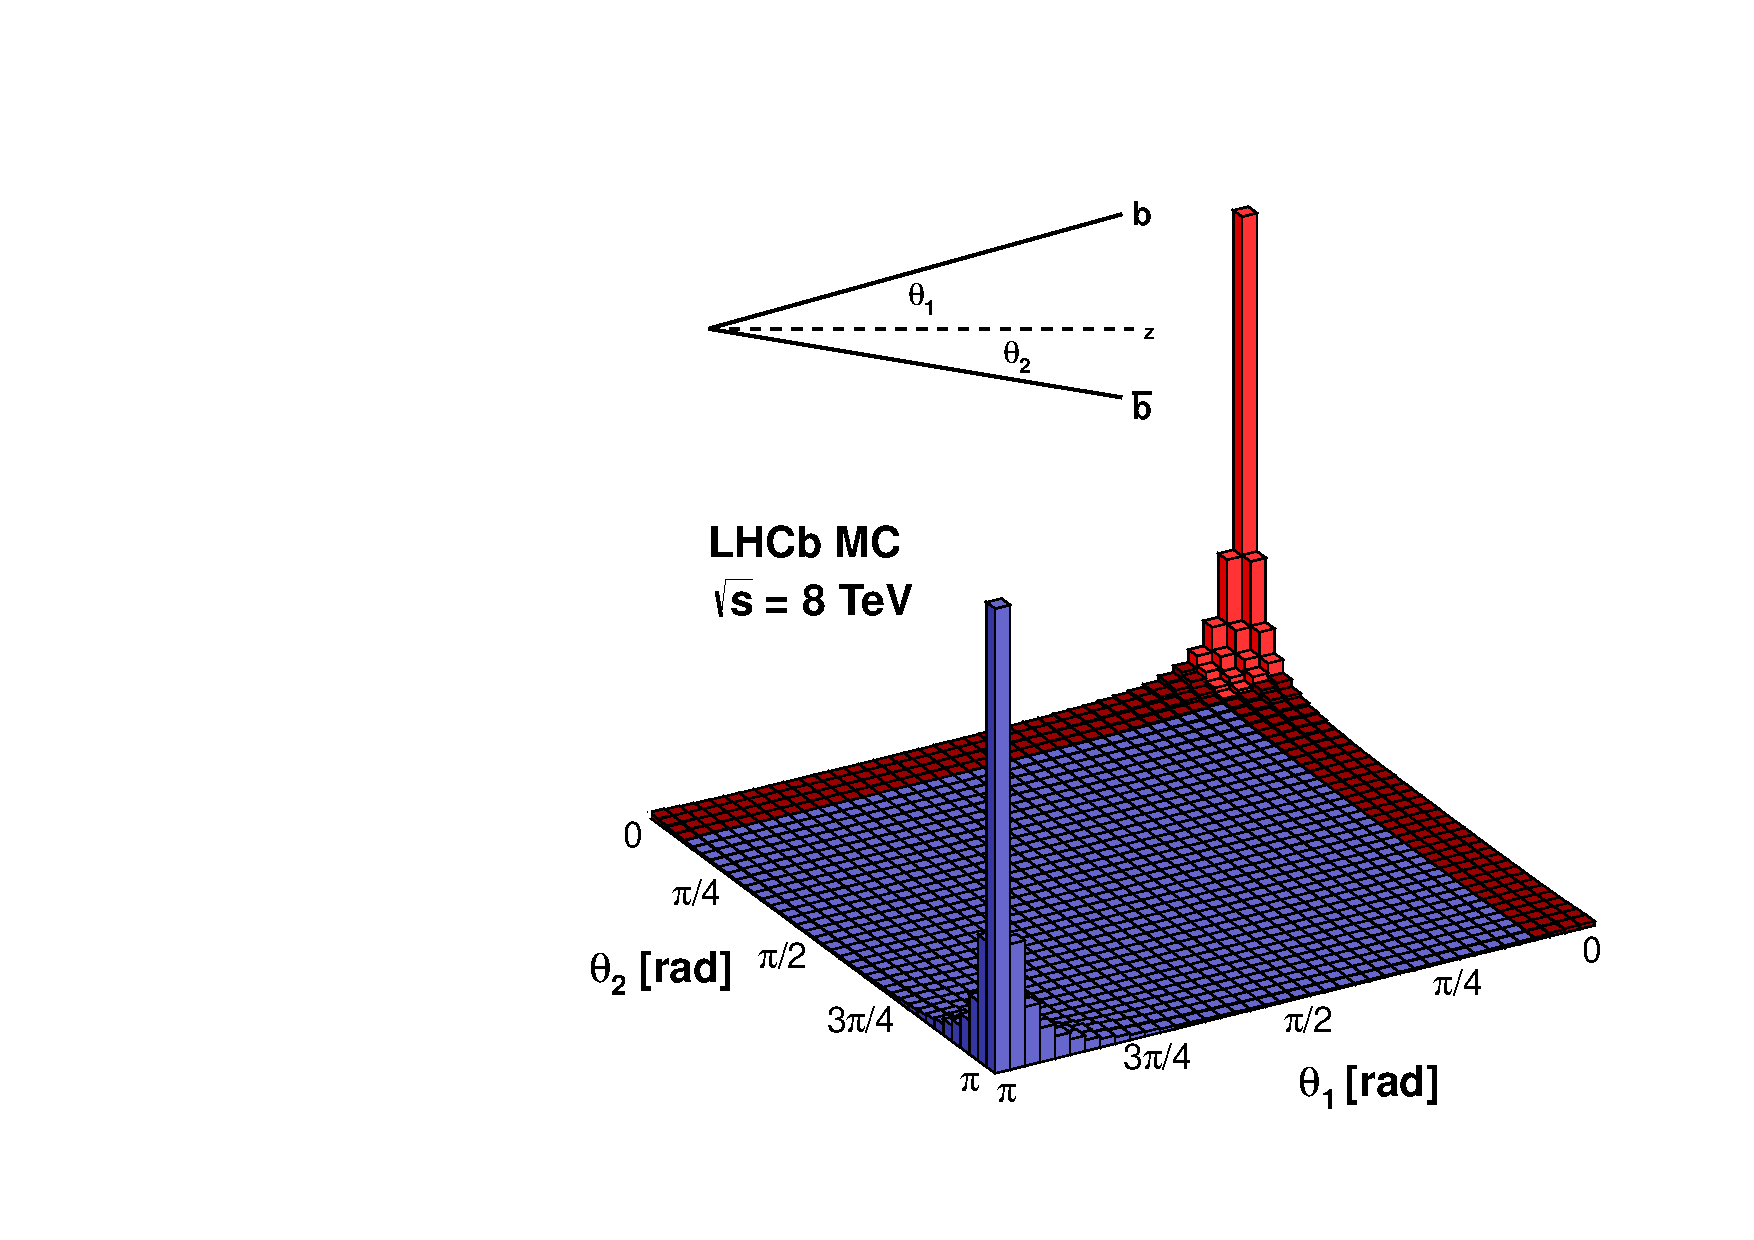
\includegraphics[width=0.5\linewidth]{figures/detector/08_rad_acc_scheme_right.pdf}
\caption{The cross-section of \bquark\bquarkbar quark pair productions in simulated $pp$ collisions at 8 TeV as a function of the polar angles $\theta_1$ and $\theta_2$ with respect to the beam axis, $z$. The red portion indicates the region covered by the \lhcb detector}
\label{bbar}
\end{figure}

\begin{figure}
\includegraphics[width=\linewidth]{figures/detector/lhcb.pdf}
\caption{Diagram of the \lhcb detector}
\label{lhcbdetector}
\end{figure}

\section{The Vertex Locator}
\label{sec:detector:velo}

The Vertex Locator (\velo)~\cite{LHCb-DP-2014-001} provides precise tracking close to the interaction point to identify primary and secondary vertices, which is essential for studies of long-lived particles such as \B and \D mesons. The \velo is a silicon microstrip detector situated around the proton-proton interaction point. It consists of 42 silicon modules arranged along the beam, each providing a measurement of the radial coordinate, $r$, and azimuthal coordinate, $\phi$, using $R$ sensors and $\Phi$ sensors respectively, shown in Figure \ref{velolayout}. The sensors are positioned 7mm from the LHC beams. The \velo modules are retracted 29mm in the horizontal direction during the injection of the LHC beams and returned to their original position during stable beams in order to reduce damage due to radiation. The sensors are enclosed in a vacuum, which is separated from the LHC vacuum by corrugated foil sheets that protect the \velo modules against electromagnetic interference from the LHC beams.

\begin{figure}
\centering
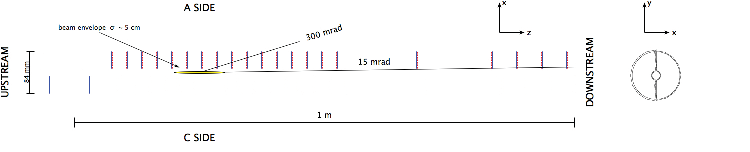
\includegraphics[width=\linewidth]{figures/detector/VELO_detector_layout_crop.pdf}
\hfill
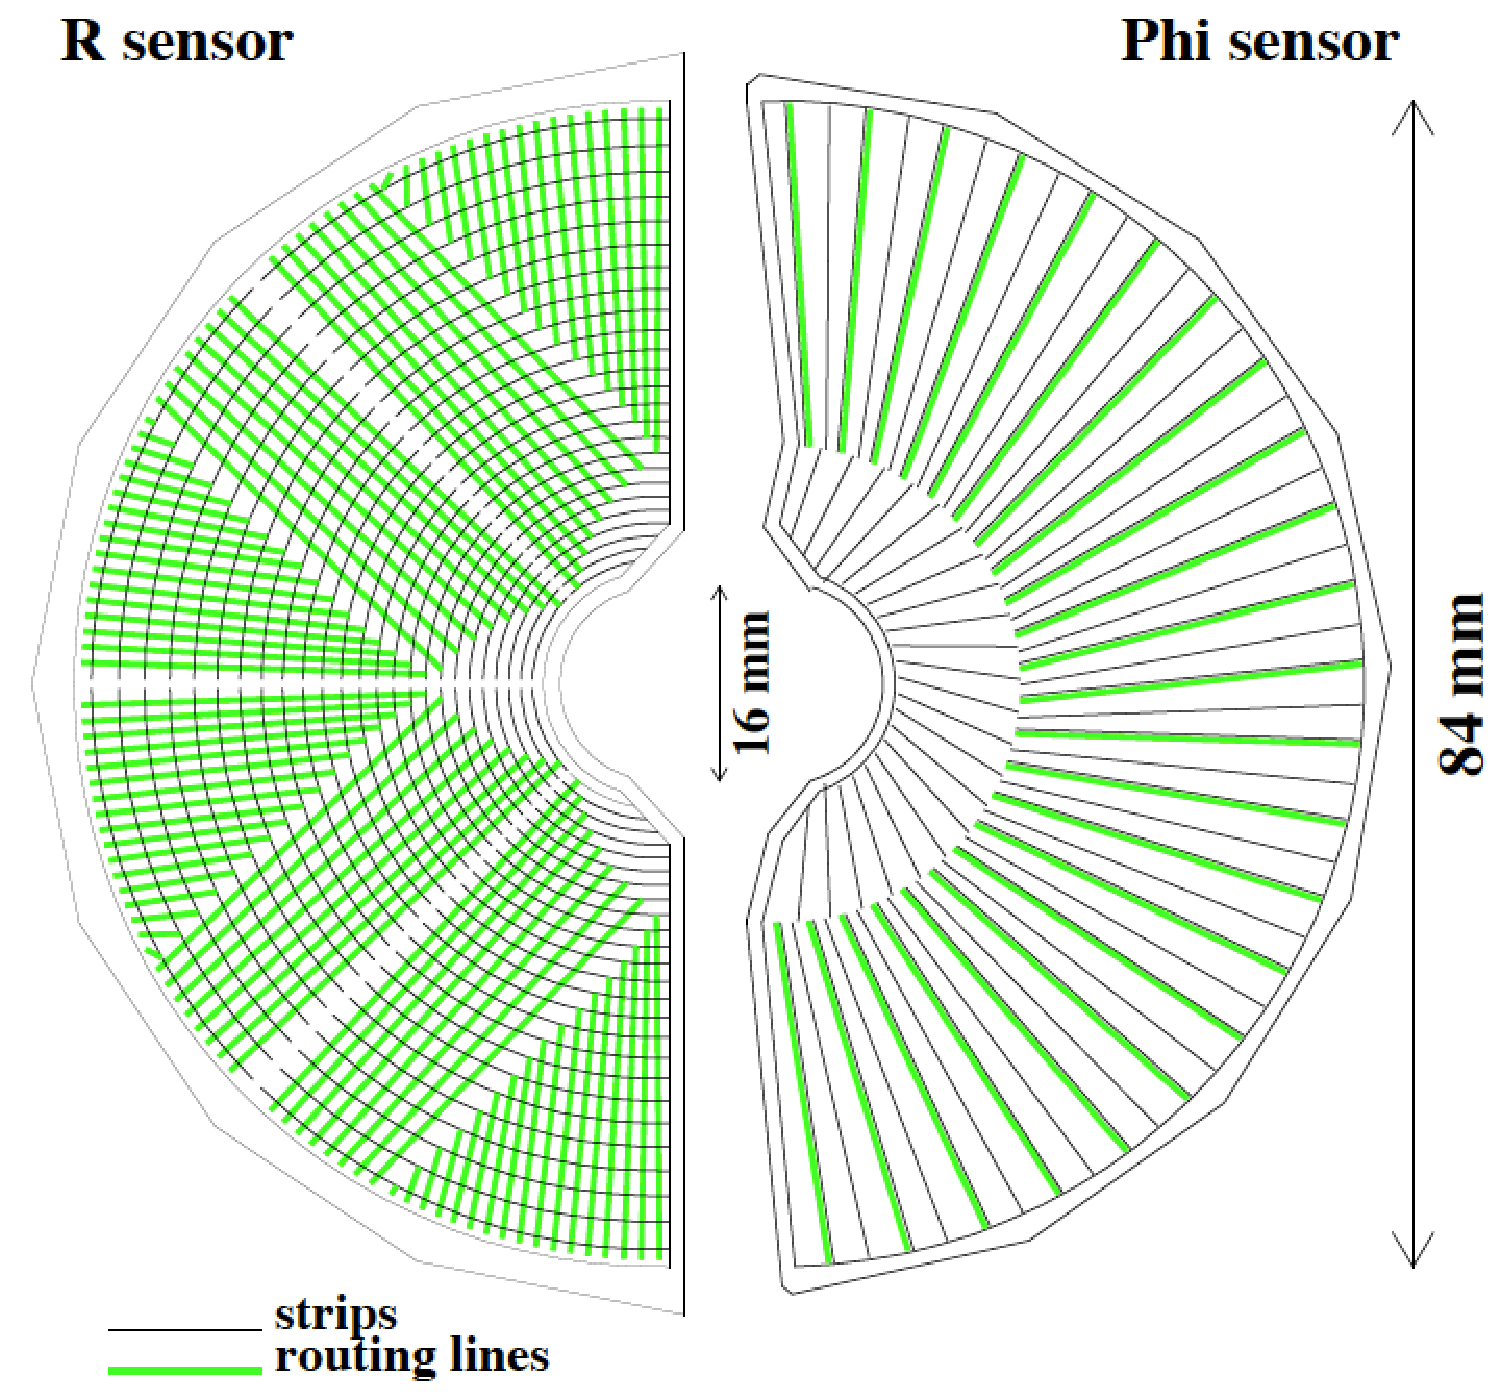
\includegraphics[width=0.3\linewidth]{figures/detector/randphisensors.pdf}
\caption{Layout of the \velo detector (top). Schematic diagram showing the $R$ and $\Phi$ sensors (bottom).}
\label{velolayout}
\end{figure}

The \velo has a high spacial resolution, enabling precise determination of a particle's flight direction close to the primary interaction point. The impact parameter (IP) of a track is defined  as the distance between the track and the PV at the track's point of closest approach to the PV. Long-lived \B and \D mesons studied in this analysis have their decay vertex displaced from the PV and as such tend to have a large IP. Therefore, the performance of the \velo can be quantified by the IP resolution~\cite{LHCb-DP-2014-001}, which, determined from 2012 data, is less than 35\mum for particles with transverse momentum greater than 1\gevc, as shown in Figure \ref{veloperformance}.

\begin{figure}
\centering
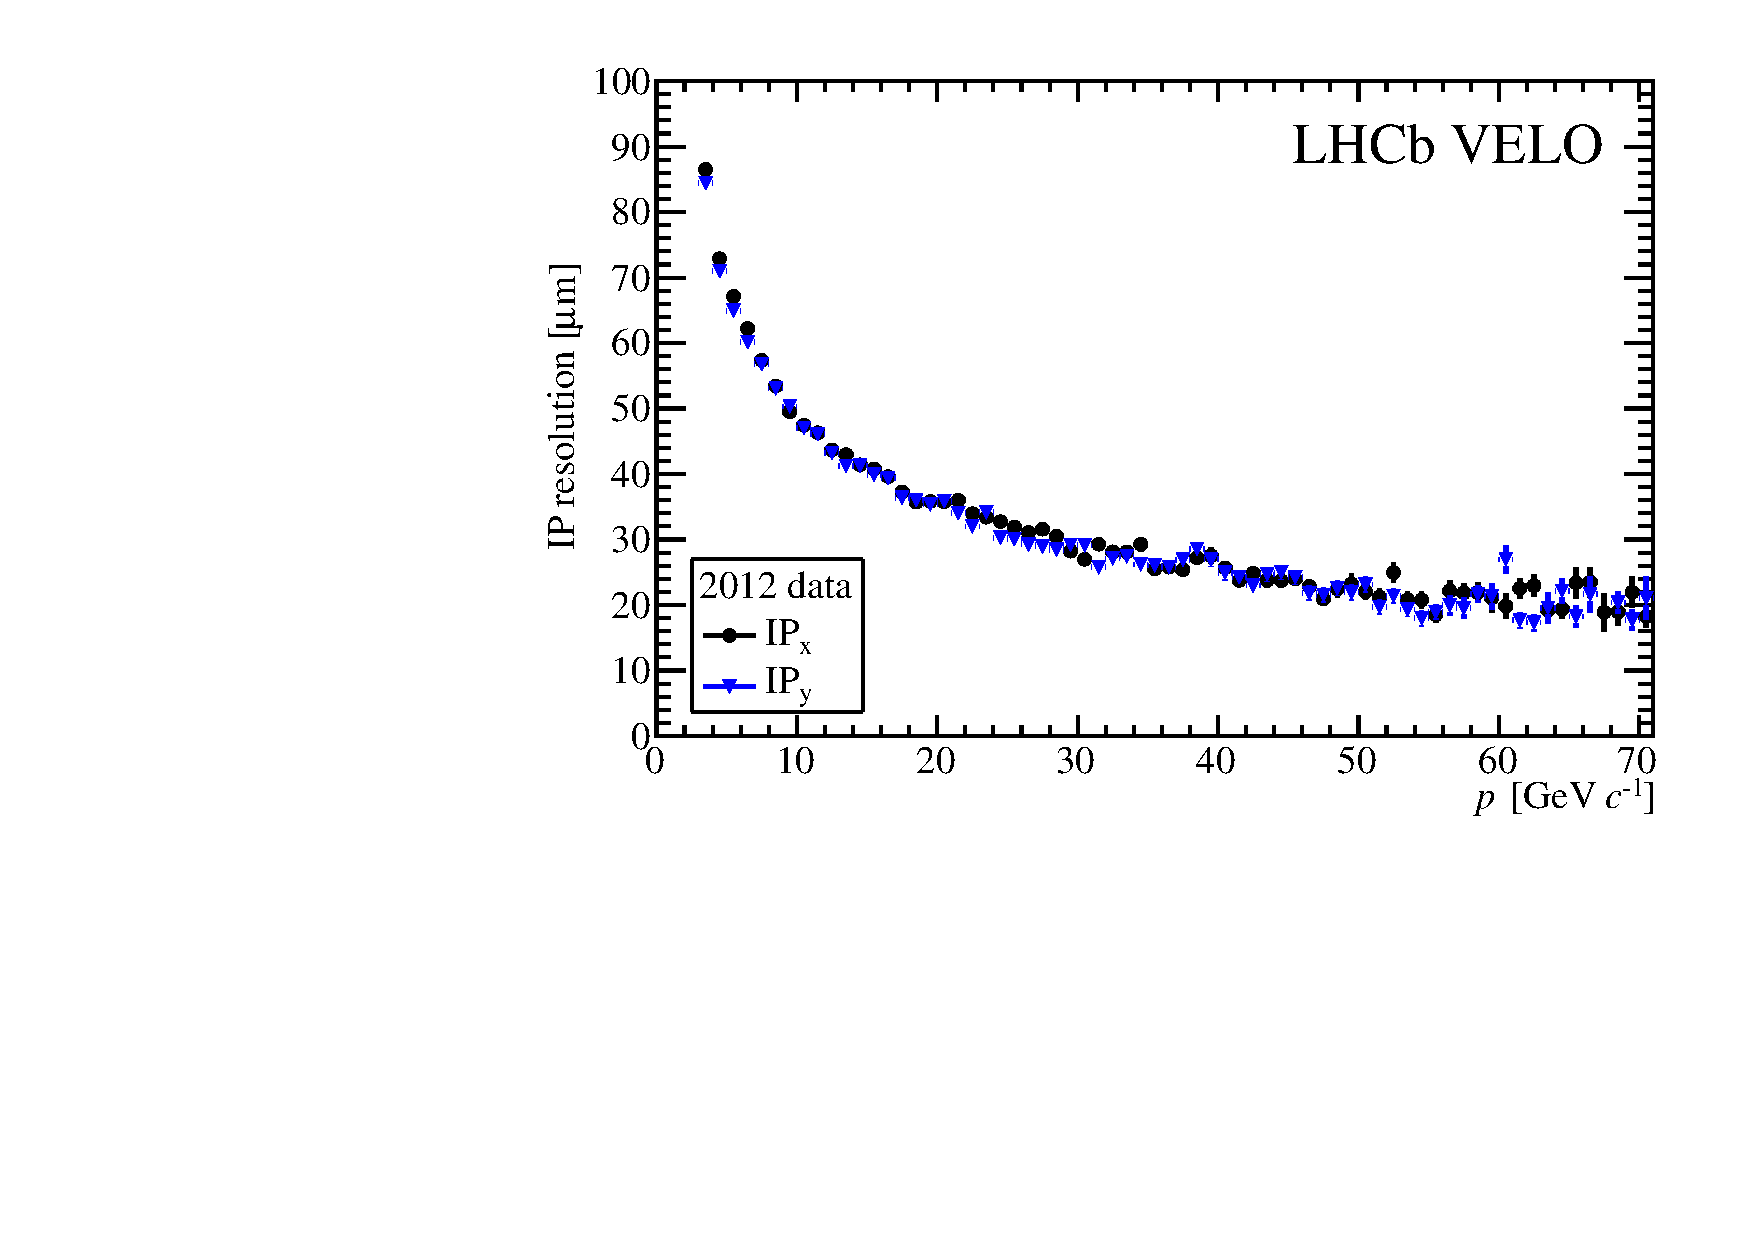
\includegraphics[width=0.5\linewidth]{figures/detector/IPRes-Vs-P-CompareIPxIPy-2012.pdf}
\caption{IP resolution as a function of momentum in both the $x$ and $y$ planes.}
\label{veloperformance}
\end{figure}

\section{Tracking and magnet}

The \lhcb tracking system consists of the \velo and four planar tracking stations further downstream: the Track Turicensis (TT) upstream of the dipole magnet, made of silicon microstrips, and tracking stations T1-T3 downstream of the magnet. The tracking stations T1-T3 have an inner region (Inner Tracker, IT) consisting of silicon microstrips, same as for the TT, and an outer region (Outer Tracker, OT) consisting of straw tubes. Charged particles require a minimum momentum of 1.5\gevc to reach the tracking stations T1-T3.

The TT and IT are constrcuted from silicon microstrip detectors. The TT is a planar detector 150\cm wide and 130\cm tall, covering the full detector acceptance with an active area of 8.4\ma. It is composed of four layers of modules with the first and fourth layers mounted vertically and the second and third layers are mounted at $+5^{\circ}$ and $-5^{\circ}$ from the vertical respectively. This gives a single hit resolution of around 50\mum. For the IT, each T-station contains four IT boxes arragned in a cross shape around the beam pipe, 120\cm wide and 40\cm tall. The OT is a straw drift tube detector. The straw tubes in each station are in four layers, with the same rotation of layers as in the TT and IT.

The dipole magnet enables the momentum of charged particles to be measured by bending the trajectory of the particles in the horizontal plane. Since positively and negatively charged particles will bend in opposite directions, a charge detection asymmetry can result if the left and right halves of the detector have different tracking efficiencies. This would affect CP violation studies, such as the one descibed in this thesis, which involve the measurements of charge asymmetries. Hence, to minimise systematics, the magnetic field direction is reversed regularly when taking data.

Performance~\cite{LHCb-DP-2013-002, LHCb-DP-2013-003}

Different reconstructed track types

\section{The \rich detectors}

The two \rich detectors (RICH 1 and RICH 2)~\cite{LHCb-DP-2012-003} are required for the identification of charged hadrons, specifically pions, kaons and protons. The decay modes of \bquark- and \cquark- flavoured hadrons involve hadronic multibody final states, making good particle identification of hadrons vital for reducing the combinatoric background. These detectors utilise the idea that Cherenkov radiation is produced whenever a charged particle, of velocity $v$, travelling through a dielectric medium, of refractive index $n$, exceeds the speed of light, $c$, in that medium. This produces a cone of light with an opening angle of $\theta_{CK}$ relative to direction of the particle's propagation, where $\theta_{CK} = \frac{1}{n\beta}$, where $\beta = v/c$. By measuring $\theta_{CK}$ as well as momentum information from the magnet and tracking systems, a mass hypothesis can be determined, as shown in Figure \ref{richseparation}.

\begin{figure}
\centering
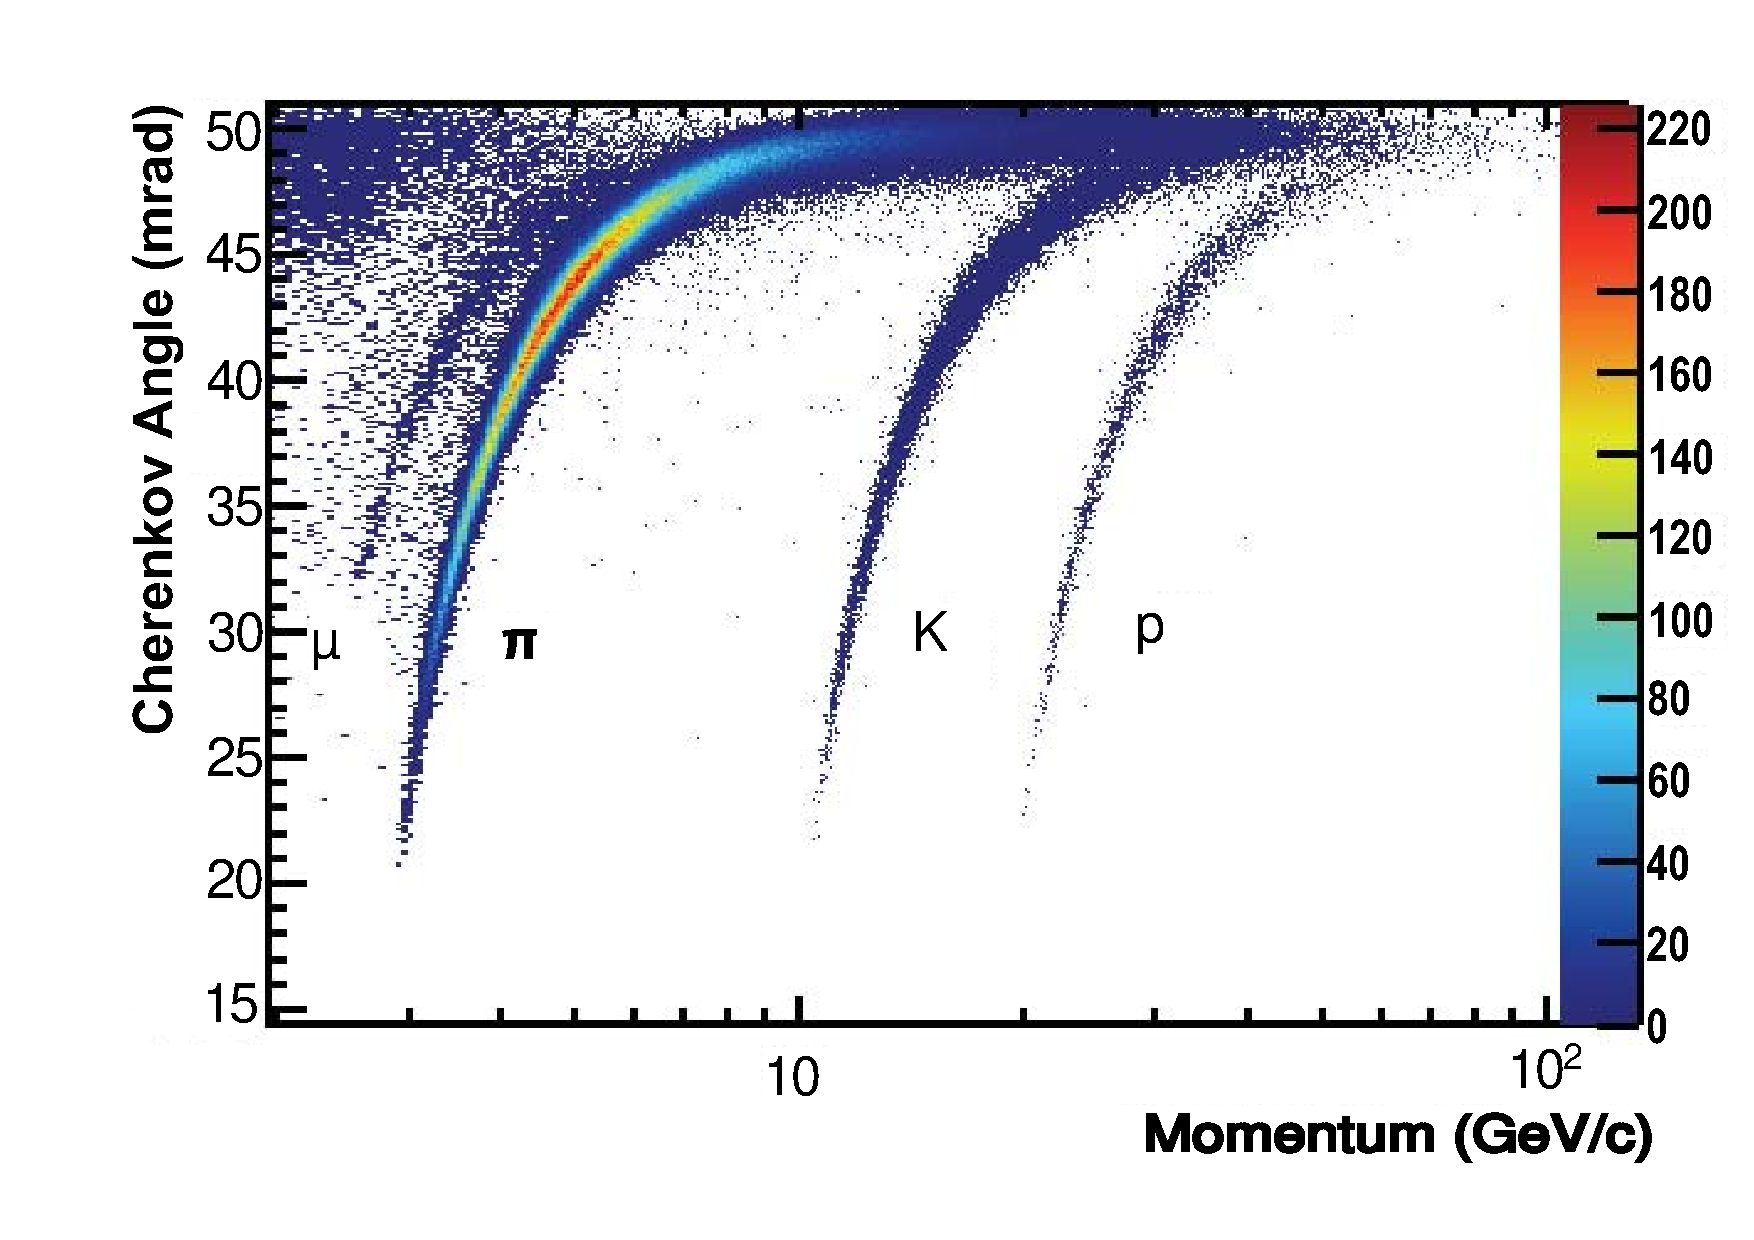
\includegraphics[width=0.8\linewidth]{figures/detector/richseparation.pdf}
\caption{Cherenkov angle as a function of momentum}
\label{richseparation}
\end{figure}

RICH 1 is positioned upstream of the magnet covering the low momentum range, 2 to 60 \gevc, and using two radiators: C$_4$F$_{10}$ and Aerogel in Run 1, and subsequently removing the Aerogel radiator for Run 2. Why? RICH 2 is located downstream of the magnet and covers the high momentum range, 15 to 100\gevc, using a CF$_4$ radiator. Refractive index of radiators. The cone of Cherenkov radiation that radiates from the charged particle is reflected by spherical focussing primary mirrors and planar secondary mirrors to form a ring on Hybrid Photon Detectors (HPDs). The value of $\theta_{CK}$ can be determined from the diameter of the ring. 

Although the RICH system is designed primarily to provide separation between charged hadrons (\pion, $K$ and $p$), it can provide some information on leptons. Similarly, the calorimeters and muon systems can provide some hadron identification. A global likelihood hypothesis for each particle type (\pion, $K$, $p$, $e$, $\mu$) is formed by combining the particle likelihood hypotheses as determined by each subdetector, $\mathcal{L}_X$ for particle hypothesis $X$. Since the most abundant particles from a $pp$ interaction are pions, the pion hypothesis is initially assumed. For each track the relative differences between a particle hypothesis, $X$, log-likelihood compared to the pion hypothesis is computed:
\begin{equation}
DLLX = \log{\mathcal{L}_X} - \log{\mathcal{L}_{\pi}} \text{ .}
\end{equation}

The performance of the \rich detectors \ref{richperformance}

\begin{figure}
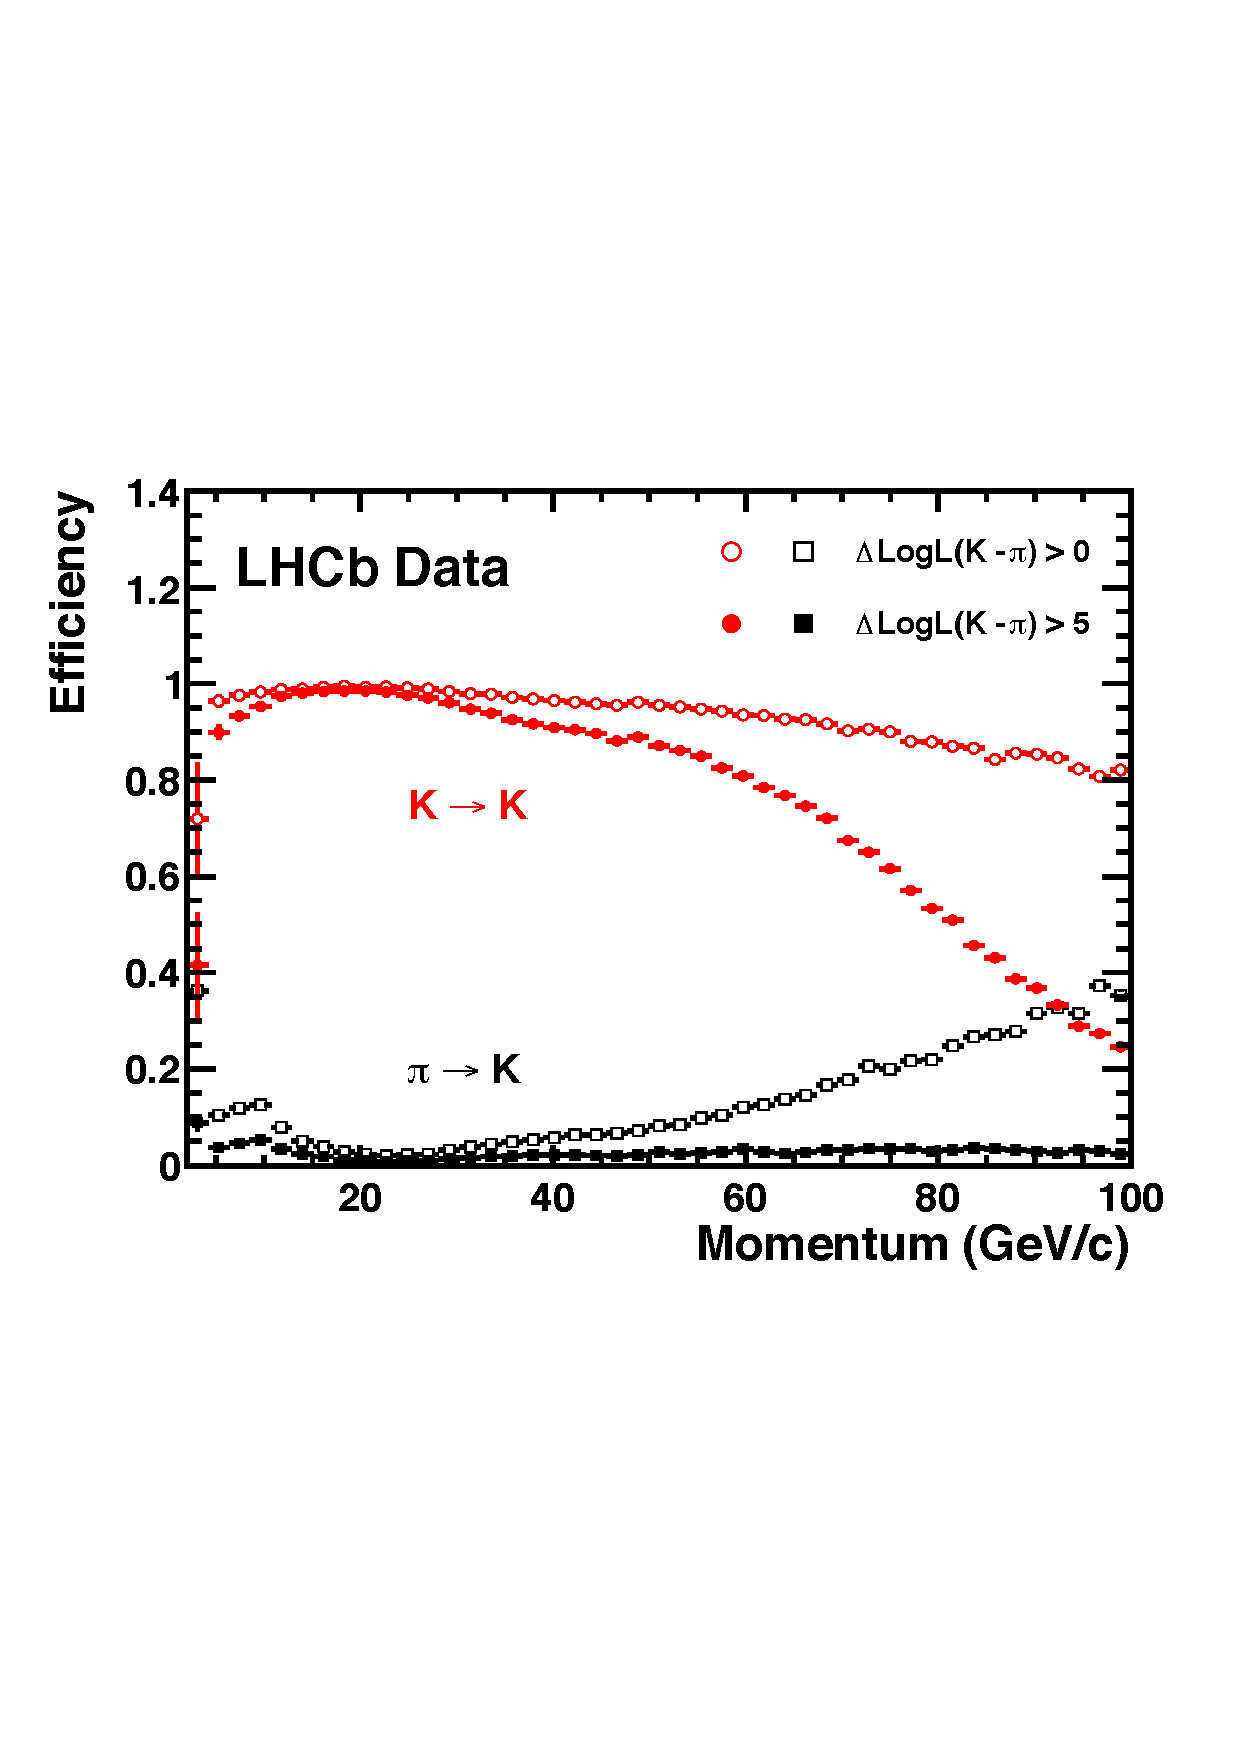
\includegraphics[width=0.5\linewidth]{figures/detector/richperformance-data.pdf}
\hfill
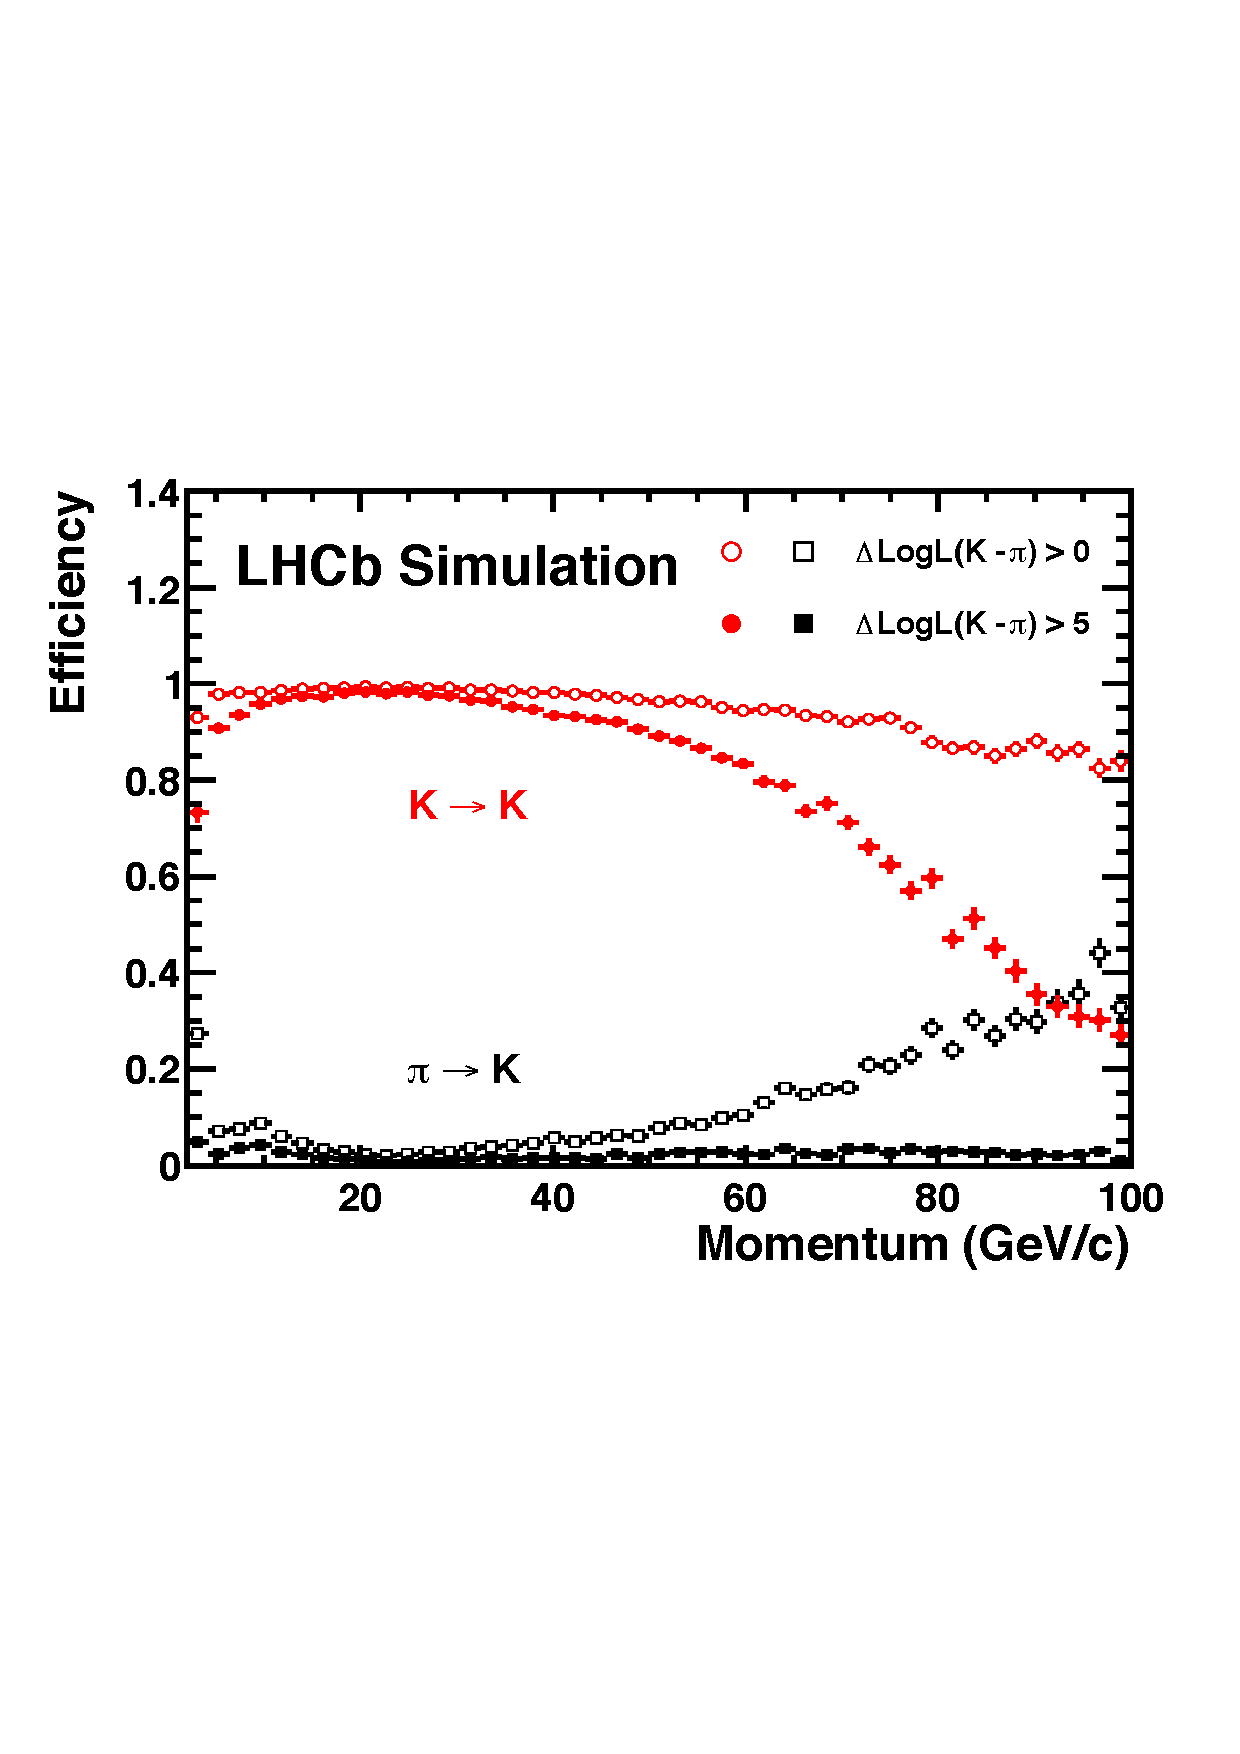
\includegraphics[width=0.5\linewidth]{figures/detector/richperformance-mc.pdf}
\caption{Plots of \rich performance}
\label{richperformance}
\end{figure}

\section{Calorimeters}

The calorimeter system provides energy measurements and is essential for the first level of the trigger to select particles with high transverse energy. It consists of four systems: the scintillating-pad (SPD) and pre-shower (PS) detectors, the electromagnetic calorimeter (ECAL) and hadronic calorimeter (HCAL)~\cite{LHCb-DP-2013-004}. The calorimeter system provides energy measurements using the mechanism of detecting scintillation light using photomultiplier tubes (PMTs) and is located downstream of RICH 2, between the first two muon stations. The ECAL is required to measure electrons and photons and the HCAL to measure charged and neutral hadrons.  The SPD/PS detectors are nearest the interaction point and designed to help the ECAL with electron identification. Between the SPD and PS is a 15\mm lead converter, 2.5 radiation lengths thick, to initiate showering before the PS. The ECAL is composed of 4\mm thick alternating lead absorber and polystyrene scintillator layers with an acceptance of 300mrad horizontally and 250mrad vertically. The thickness of the ECAL corresponds to 25 radiation lengths, chosen to fully contain high energy photon showers for optimum energy resolution. The HCAL has the scintillating tiles mounted parallel to the beam axis to increase the contact area between the scintillator tiles and optical fibres maximising the amount of scintillation light collected. The polystyrene scintillator tiles are separated by 100m thick iron absorber plates. The HCAL has a thickness limited to 5.6 nuclear interaction lengths due to space limitations. The measured energy resolution is $\sigma_E/E = (69 \pm 5)\%/\sqrt{E} \oplus (9 \pm 2)\%$ for $E$ in \gev.

All four components of the calorimeter system are composed of scintillator pads with a cell granulartity that decreases moving outwards, away from the beam pipe. The SPD/PS and ECAL have the variable segmentation split in to three sections, whereas the HCAL is split into two zones with larger cell sizes due to the larger size of hadronic showers.

\section{Muon systems}
\label{sec:detector:muon}

The muon system~\cite{LHCb-DP-2013-001,LHCb-DP-2012-002} is designed, together with the calorimeter system, to provide information to the first level hardware trigger. It is composed of five stations, labelled M1 through to M5. Station M1 is located upstream from the calorimeteres and is only used in the first level trigger. Stations M2 - M5, located downstream from the calorimetersm, are interleaved with 80\cm thick iron absorbers and are designed to identify and trace penetrating muons. muons with momenta greater than 6\gevc will typically traverse all five stations. The five stations together have a width corresponding to 20 interaction lengths. 

Each stations uses multiwire proportional chambers (MWPCs) apart from the inner most region of M1, which consists of gas electron multipliers (GEMs) due to their radiation hardness. Stations M1 to M3 have the best spatial resolution and measure transverse momentum with a resolutions of 20\%.

\section{Trigger system}

The \lhc bunch crossing rate is 40MHz, however there is insufficient processing power to read out the full detector and write every event to storage. A dedicated trigger system~\cite{LHCb-DP-2012-004} is implemented to retain interesting events while discarding background events. This occurs in two stages, the low level hardware trigger, called Level-0 (L0), and the high level software trigger, called High Level trigger (HLT). The L0 trigger operates at the bunch crossing rate of 40MHz, reducing the event rate to 1MHz. The HLT only processes events that have passed L0, accepting events at a rate of 3kHz.

A sequence of reconstruction algorithms and thresholds defined in the trigger to select a specific decay is called a trigger line. This returns an accept or reject decision. An event is retained only if it passes at least one trigger line in both L0 and HLT.

\subsection{Level-0 trigger}

The L0 trigger only uses information that can be quickly read out from the calorimeter or muon systems, reducing the event rate from 40MHz to 1MHz, at which point the full detector is read out. The decay products of \B mesons typically have high transverse energy and momentum due to the large \B mass. Selections are made on global quantities. The L0 trigger selects high transverse energy clusters in the calorimeters due to hadrons, photons and electrons, and high transverse momentum muons in the muon system. The trigger also requires a maximum number of SPD hits to reject high multiplicity events which would use excessive processing time in HLT. The trigger creates {\tt L0Hadron}, {\tt L0Photon} or {\tt L0Electron} candidates depending on where the energy has been depositied in the calorimeter. Events containing at least one candidate above the fixed threshold in transverse energy required are accepted by the L0 trigger. Candidates for {\tt L0Muon} or {\tt L0DiMuon} are also created based on the hits in the muon systems and the transverse momentum of the candidate.

\subsection{High Level Trigger}

Events accepted by the L0 trigger are placed in a buffer to be processed by HLT, which has two stages: HLT1, performing partial event reconstruction, and HLT2, performing full event reconstruction. For HLT1, the event rate has been reduced to 1MHz allowing for the full detector to be read out.

In HLT1, tracks in the \velo are reconstructed and are then used to construct vertices using at least five tracks. HLT1 lines that do not require muons select \velo tracks based on their smallest impact parameter to any PV. Poor quality \velo tracks are rejected. Muon candidates are selected by matching \velo tracks to those events triggered by {\tt L0Muon} or {\tt L0DiMuon} with the additional requirements of high momentum (above 6\gevc) and reasonable track quality (\chisqndf below 25). \velo tracks that are selected by their IP or as a muon candidate are reconstructed using information from the OT and IT-stations in order to determine their momentum. This process is known as forward tracking. Minimum momentum and transverse momentum constraints are applied to reduce processing time when fitting each reconstructed track using a Kalman filter based track fit. Selections are applied to the IP, momentum and mass of the candidates.

In HLT2, the further reduction is event rate allows forward tracking to be performed on all \velo tracks with $p > 5\gevc$ and $\pt > 0.5gevc$. The HLT2 trigger includes trigger lines for selecting \bquark-hadron decays, prompt charm decays and muonic decays. A large proportion of the HLT2 bandwidth goes to topological trigger lines, which are specifically designed to target partially reconstructed \bquark-hadron decays. Tracks are then combined one-by-one requring the distance of closest approach (DOCA) to be less than 2mm, reaching a total of two, three or four tracks, resulting in the {\tt HLT2Topo(N)BodyBDTDecision} trigger lines, where $N = 2,3,4$ particles forming the vertex. Selection requirements are imposed on these lines based on a multivariate Boosted Decision Tree (BDT) classifier, which uses the sum of transverse momenta, minimum transverse momenta, mass, $m_{corr}$, DOCA, impact parameter significance and flight distance significance, where $m_{corr}$ is the corrected mass, defined as

\begin{equation}
m_{corr} \equiv \sqrt{m^2 + {| \pt^{miss} |}^2} + \pt^{miss} \text{ ,}
\end{equation}

where $\pt^{miss}$ represents the missing momentum in the transverse direction. This quantity allows for the case where not all final state particles are reconstructed. 

Events that pass HLT2 are written to storage at an event rate of about 3kHz. These events subsequently undergo the full alignment, calibration and reconstruction processes.

\section{Reconstruction}

\subsection{Track reconstruction}

Track reconstruction algorithms combine information of hits from different sub-detectors, e.g. \velo, TT, IT and OT. There are five catergories for track classification, shown in Figure \ref{tracktypes}:

\begin{figure}[h]
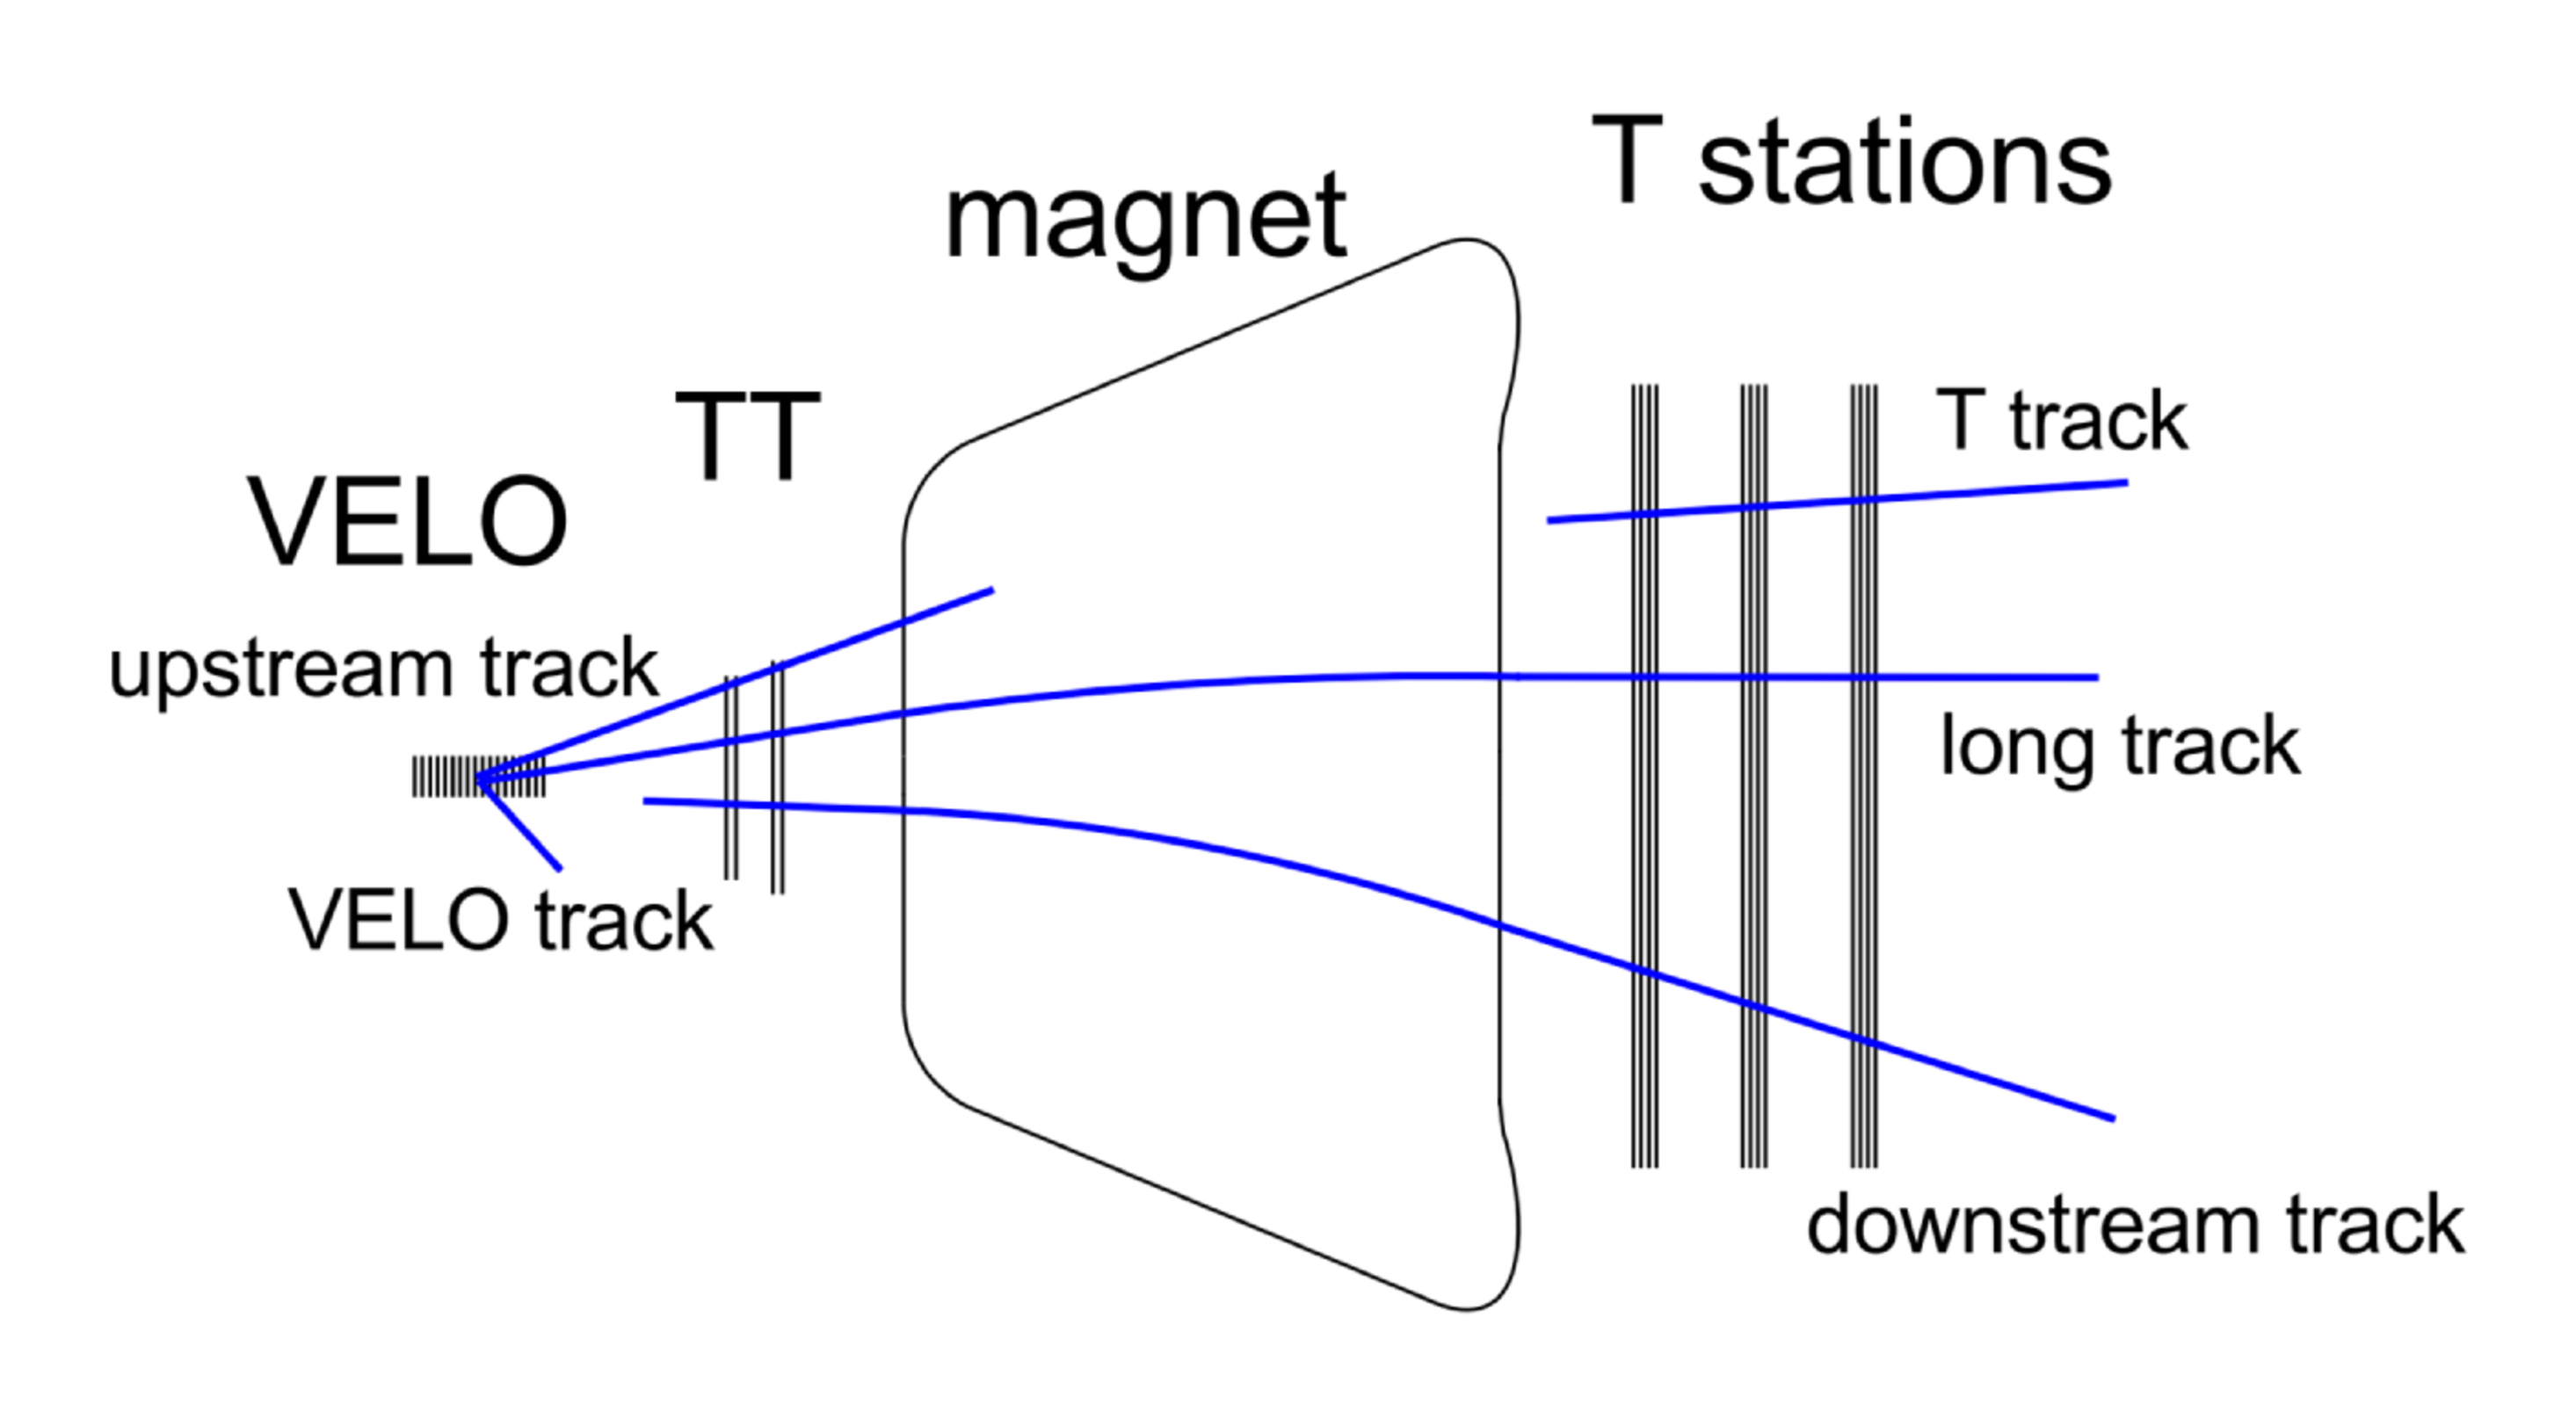
\includegraphics[width=\linewidth]{figures/detector/tracktypes.pdf}
\caption{Schematic diagram of the different tracking sub-detectors (\velo, TT, T-stations) and the different categories of reconstructed tracks (long, downstream ,upstream, \velo, T tracks).}
\label{tracktypes}
\end{figure}

\begin{itemize}
\item \textbf{Long tracks} traverse the entire tracking system from the \velo to the T-stations. These tracks have the most precise momentum measurement as they have experienced the full magnetic field.
\item \textbf{Downstream tracks} only traverse the TT and T-stations. These tracks are usually due to the presence long-lived particles, such as \KS mesons, decaying after the \velo.
\item \textbf{Upstream tracks} traverse the \velo and TT stations before being bent out of the detector by the magnetic field due to their lower momentum.
\item \textbf{\velo tracks} leave the \lhcb acceptance after traversing part of the \velo. No momentum information can be pbtained from these tracks due to the absense of a magentic field.
\item \textbf{T tracks} are one that only measure hits in the T-stations. These are typically produced in secondary interactions.
\end{itemize}

Track reconstruction starts with the reconstruction of \velo tracks, which are then propagated through to the TT to determine the particle trajectory. To define a long track, additional hits are searched for in the T-stations that match the partcle trajectory. This process finds combinations of clusters in different sub-detectors that are likely to have been fromed by a single charged particle travelling though the detector. The clusters are then fit with a \chisq fit using a third order polynomial. Downstream tracks are reconstructed by first searching for T tracks and then finding corresponding hits upstream in the TT by extrapolating the track trajectory through the magnetic field.

The tracks are fitted to obatin a best estimate of the track parameters accounting for multiple scattering and energy lost through ionisation. The \chisq of this fit and a neural network classifier are used to reduce the number of fake tracks that are formed by wrongly matching clusters in different sub-detectors, and therefore do not correspond to the track of a real charged particle.

%\subsection{Particle identification}
%
%Discussion of DLL variables. Already in \rich section?

\subsection{Stripping}

The events accepted by the trigger are written to storage. All processing that occurs after this point is known as ``offline''. These events are processed with more accurate alignment and calibration of the sub-detectors and more sophisticated reconstruction software than HLT. This offline processing stage is known as stripping. Each family of decays has its own stripping line, which refers to the reconstruction and selection of specified particles in the decay chain of interest. Various loose selection requirements are applied in the stripping line to reduce remove background event while reducing the processing time and storage requirements. An analysis initially involves taking events returned by the relevant stripping line and developing a more sophisticated selection procedure to further remove background events. The stripping lines used in this analysis are listed in Section \ref{sec:selection:strippingandtrigger}.

\section{Simulation}

Various simulated samples were generated for signal and background studies. The simulated samples are generated using the \lhcb application \gauss and \boole, which are written using the \gaudi framework. \gauss generates particles and their decays as well as simulating the transport through the detector. \boole is then used to simulate the detector response. 

In the production of simulation samples used for analysis, the first step is the production of \bquark\bquarkbar pairs is simulated from $pp$ collisions using \pythia. One quark in the \bquark\bquarkbar pair is chosen to decay at random via user-specified process and its decay is simulated using \evtgen, with \photos modelling any final state radiation. The transport of the decay through the detector is modelled using \geant. 

\boole is then used to simulate the detector response and return the output in the format of real data coming from the front end electronics. The simulated data is then processed by the trigger, reconstruction and stripping as for real data.

Both magnet polarities, and 2011, 2012, 2015 and 2016 samples were generated with \pythia 8. All simulated samples were generated with all daughters in \lhcb acceptance. Signal samples are simulated \btodkst decays with the \Kstarm forced to \KS$\pim$ and various \D final states. For the four-body \D final states, the simulated samples are produced assuming the \D decay is uniform over the whole phase space. Many other samples are generated to investigate various possible background decays.
